%! Author = jaroslav
%! Date = 15.04.20
%%%%%%%%%%%%%%%%%%%%%%%%%%%%%%%%%%%%%%%%%%%%%%%%%%%%%%%%%%%%%%%%%%%%%%%%%%%%%%%%%%%%%%%%%%%%%%%%%%%%
%%%%%%%%%%%%%%%%%%%%%%%%%%%%%%%%%%%%%%%%%%%%%%%%%%%%%%%%%%%%%%%%%%%%%%%%%%%%%%%%%%%%%%%%%%%%%%%%%%%%
\section{Модель социально-значимых Интернет ресурсов}

Прежде чем переходить к рассмотрению квантово-подобных моделей принятия решений в условиях неопределенности,
необходимо рассмотреть классические модели, не использующие квантовый формализм. Особенность следующей модели
заключается в том, что ее модель схожа с квантовыми, но не рассматривает остальные социальные задачи, из-за чего
данная модель ограничена в применении.
Это модель социально-значимых Интернет ресурсов, разработанная на основе результатов исследований в социальной
психологии, в механизме запоминания информации человеком, а также на основе теории информации~\citep{pilkevich2015model}.
Данная модель в равной степени адекватно описывает поведение участников сети Интернет ресурсов.

Существует большое количество различных социальных Интернет-ресурсов.
И в первую очередь это различые социальные сети, благодаря которым человек получает персонифицированную информацию
как о себе, так и о других участниках.
Это блоги, благодаря которым человек получает более развернутую информацию.
Различные форумы, которые позволяют обсуждать некоторыую тему и др.
Для предоставления участникам ресурса возможности общения, во многих Интернет-ресурсах требуется предварительная
регистрация.
Определенного шаблона для составления анкеты на этапе регистрации не существует, поскольку различные Интерент-ресурсы
требуют не все данные о пользователе.
Однако, существует некоторая тенденция в составлении анкет во время регистрации, благодаря чему можно спроектировать
модель аккаунта пользователя.

В модели социально-значимых Интернет-ресурсов предлагается модель пользовательского аккаунта.
Эта модель описывает большое количество различных параметров анкеты пользователя.
Эта модель имеет следующий вид:
\begin{equation}
    A = <Pers, Cont, CoC, Prof>,
\end{equation}
где $Pers$ — подмножество идентифицирующей информации, $Cont$ — подмножество контактных данных,
$CoC$ — подмножество данных о социальных связях, $Prof$ — подмножество различной личной информации.

Помимо этого, для этой модели существует модель распространения информации, которая имеет вид:
\begin{equation}
    I = <Pers, M, T>,
\end{equation}
где $Pers$ — подмножество идентифицирующей информации, $M$ — мнения, комментарии,
$T$ — отметка времени, $K = f(M)$ — когниция, элемент знания (данные, усвоенные сознанием).

Помимо этого, модель пользовательского аккаунта имеет информацию о связях с другими аккаунтами,
которая позволяет рассчитать параметр интенсивности отношений:
\begin{equation}\label{alphaik}
    \alpha_{ik} = N log_{2} \frac{N_{ik}}{N_{0}},
\end{equation}
где $N_{ik}$ – количество переданых сообщений/знаков между членами $i$ и $k$,
$N_{0}$ – среднее значение переданных сообщений в сообществе, $N$ – некоторая константа, различная для каждого индивида.

На основе формулы \ref{alphaik}, а также модели пользовательского аккаунта и модели распространения информации
приводится схема взаимодействия пользователей и информации в виде графа (см. рисунок \ref{fig:shema_system_in_socium}).

\begin{figure}[h!]
    \centering
    \captionsetup{justification=centering}
    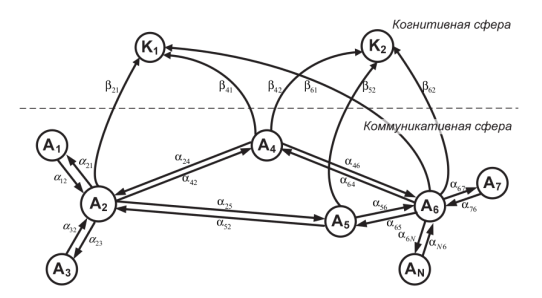
\includegraphics[width=0.8\linewidth]{pictures/schema_system_in_socium.png}
    \caption{Схема системы психологических отношений в социуме (социально значимых Интернет-ресурсах)}
    \label{fig:shema_system_in_socium}
\end{figure}

На этом рисунке $A = \{ A_{1}, A_{2}, A_{3}, \dots, A_{N}\}$ – это члены сети,
$K = \{ K_{1}, K_{2}, K_{3}, \dots, K_{N}\}$ – это когниции.~Схема построена с учетом теории когнитивного
~диссонанса Л.~Фестингера,~теории структурного баланса Ф.~Хайдера, теории коммуникационных актов Т.~Ньюкома
и теории конгруэнтности Ч.~Осгуда и П.~Танненбаума, для которых базовыми постулатами являются предположения
о возможности получения человеком информации, его переработке, его усвоению, о стремлении человека к наибольшей
связности имеющихся знаний, которые могут побуждать к действиям.

Самым~простым элементом отношений в этой схеме является рассмотрение двух членов социума (O,S) и одной когниции (K).
Смена значений этих отношений называется как информационно-психологическая акция (ИПА).
Данная ИПА представлена на Рисунке~\ref{fig:shema_OSK}.
\begin{figure}[h!]
    \centering
    \captionsetup{justification=centering}
    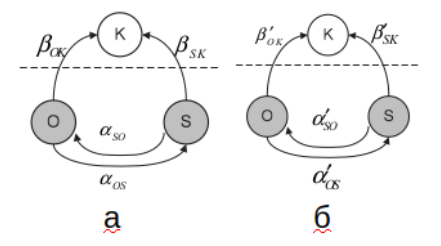
\includegraphics[width=0.7\linewidth]{pictures/schema_OSK.png}
    \caption{Схема отношений объекта O и субъекта S друг к другу и к утверждению K: a)
    для события до ИПА; б) после ИПА~\citep{pilkevich2015model}}
    \label{fig:shema_OSK}
\end{figure}
На рисунке~\ref{fig:shema_OSK}~а параметры $\alpha_{OS}, \alpha_{SO}$ показывают отношение объекта и субъекта
друг к другу, параметры $\beta_{OK}, \beta_{SK}$ показывают отношение членов социума к утверждению.
На рисунке~\ref{fig:shema_OSK}~б, эти отношения имеют новые значения и обозначаются
$\alpha^{\prime}_{OS}, \alpha^{\prime}_{SO}, \beta^{\prime}_{OK}, \beta^{\prime}_{SK}$
Изменение значений для параметров отношений вычисляются на основе дифференциалов Осгуда и для этой модели
записываются следующим образом:
\begin{equation}
    \Delta_{OK} = \frac{|\alpha_{OS}|}{|\beta_{OK}|+|\alpha_{OS}|} |\beta_{OK}-\alpha_{OS}|,\\
    \Delta_{OS} = \frac{|\beta_{OK}|}{|\beta_{OK}|+|\alpha_{OS}|} |\beta_{OK}-\alpha_{OS}|
\end{equation}
где $\Delta_{OK}, \Delta_{OS}$ – это приращение к $\beta_{OK}, \alpha_{OS}$ соответственно.
Различные ситуации взаимоотношений между элементами {O,S,K} были рассмотрены в теории структурного
баланса Ф.~Хайдера, а изменение отношений рассмотрено в теории коммуниуативных актов Т.~Ньюкомба,
благодаря чему известны формулы для $\beta^{\prime}_{OK}, \alpha^{\prime}_{OS}$, которые получаются
от начальных параметров отношений $\beta_{OK}, \alpha_{OS}$ и приращений к ним $\Delta_{OK}, \Delta_{OS}$.

В работах по моделированию информационно-психологических отношений наблюдается явление, при котором
элемент социума при получения некоторой когниции распространяет его вторично.
Формула, по которой это вторичное распространение информации описывется имеет вид:
\begin{equation}\label{beta_ij}
    \beta_{ij}(t) = \beta_{ij}(t_0)\cos(\rho_{i}\sqrt{t-t_0})e^{-\lambda_{i}(t-t_0)},
\end{equation}
где $t_0$ – время последнего изменения отношения элемента социума к когниции (утверждению), $t$ – текущее
время изменения, $\lambda_{i}$ – коэффициент «старения и утраты уникальности утверждения», $\rho_{i}$ –
коэффициент когнитивного «резонанса», вторичного распространения информации.
График данной функции представлен на рисунке~\ref{fig:graphic_beta}
\begin{figure}[h!]
    \captionsetup{justification=centering}
    \begin{minipage}[h]{0.4\linewidth}
        \center{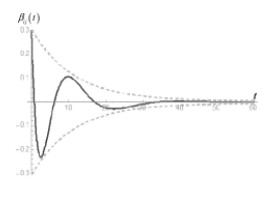
\includegraphics[width=1\linewidth]{pictures/graphic_beta_a.png} \\ а)}
    \end{minipage}
    \hfill
    \begin{minipage}[h]{0.4\linewidth}
        \center{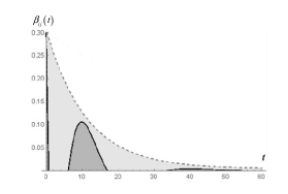
\includegraphics[width=1\linewidth]{pictures/graphic_beta_b.png} \\ б)}
    \end{minipage}
    \caption{Уровень отношения $\beta_{ij}(t)$ члена сети $A_{i}$ к утверждению $K_{j}$~\citep{pilkevich2015model}}
    \label{fig:graphic_beta}
\end{figure}

Данный график, к сожалению, не показывает других зависимостей этой функции от других параметров, но
на нем хорошо видно как ведет функция себя при постоянных параметрах.
На рисунке~\ref{fig:graphic_beta}а показан полный вариант с положитеьлными и отрицательными полупериодами.
Отрицательные полупериоды показывают маловероятное проявление когнитивной активности.
Положительные полупериоды показывает наиболее вероятное проявление когнитивной активности.
Для более детального рассмотрения графика функции $\beta_{ij}(t)$, на рисунке~\ref{fig:beta_another_param}
представлены зависимости с дополнительным параметром ($\lambda_{i}$).
\begin{figure}[h!]
    \centering
    \captionsetup{justification=centering}
    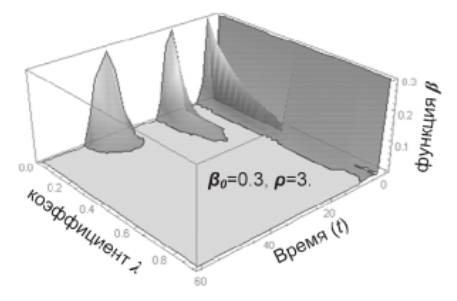
\includegraphics[width=0.7\linewidth]{pictures/graphic_beta_anotherparam.png}
    \caption{График функции когнитивной активности $\beta_{ij}(t)$ в зависимости от динамики параметра $\lambda_{i}$~\citep{pilkevich2015model}}
    \label{fig:beta_another_param}
\end{figure}

Как видно из этого и предыдущего графиков, что существуют семейства монотонно убывающих зависимостей
Эббингауза при определенных значениях параметра $\lambda_{i}$.
Однако, как подчеркнули сами авторы, данную модель невозможно использовать в практической деятельности,
но предлагают ограничение этой модели в определенных коэффициентах для определенных однородных групп,
иначе говоря групп состоящих из людей с одним уровнем образования или предпочтений.
Таким образом диапазон модели для $4.5 < \rho_{i} < 5$ представлен на рисунке~\ref{fig:beta_4_5rho5}
\newpage
\begin{figure}[h!]
    \centering
    \captionsetup{justification=centering}
    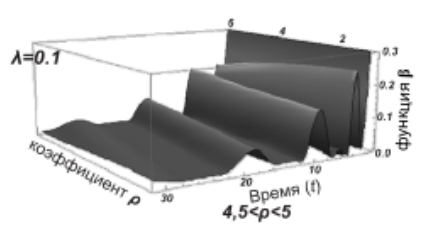
\includegraphics[width=0.7\linewidth]{pictures/graphic_beta_45rho5.png}
    \caption{График функции диффузной активности $\beta_{ij}(t)$ в зависимости от динамики параметра $\rho_{i}$~\citep{pilkevich2015model}}
    \label{fig:beta_4_5rho5}
\end{figure}

В работе утверждается, что данное поведение похоже на социальную диффузию, которое представляется как
\glqqкогнитивный шум\grqq.
Интересно также то, что данный шум показывает момент перехода мнения человека к мнению группы, что так
же подтверждает справедливость уменьшения диапазонов $\rho_{i}$ и $\lambda_{i}$.

Теперь рассмотрим эту проблему с точки зрения известных квантово-подобных моделей.
%\section{Пояснение связей экспериментов и модели}
%Связь между моделью социално-значимых Интернет ресурсов и когнитивными экспериментами заключается в
%вывляении общих рассматриваемых объектов.
%Такими объектами в экспериментах является человек или два человека и некоторый вопрос или утверждение,
%а в модели имеются два человека и утверждение.
%Это значит, что множество объектов для экспериментов и для модели имеет одну и ту же структуру.
%Схема этой структуры представлена на рисунке~\ref{fig:chain_struct}
%\begin{figure}[h!]
%    \centering
%    \captionsetup{justification=centering}
%    \includegraphics[width=0.5\linewidth]{pictures/chain_struct.png}
%    \caption{Человек и утверждение}
%    \label{fig:chain_struct}
%\end{figure}
%
%В~данном~случае~человек (агент) находится внутри~этой когниции (утверждения), таким образом агент
%воспринимает когницию как окружающий мир.
%Взаимодействие между агентом и когницией подчинятеся модели социально-значимых ресурсов~\eqref{beta_ij}.
%Причина, по которой не указано два агента, заключается в отсутствии влияния другого агента на когницию.
%Влияние агента на когницию не происходит, а происходит изменение только отношения агента к когниции.
%Это легко заметить в окружающем мире, факты о каком-либо событии невозможно изменить, их можно только
%поменять или не указывать.

\chapter{КВАНТОВЫЕ МЕТОДЫ ПОСТРОЕНИЯ МОДЕЛЕЙ ПРИНЯТИЯ РЕШЕНИЙ В УСЛОВИЯХ НЕОПРЕДЕЛЕННОСТИ}

\section{Открытые квантовые системы}

Это такая система, которая может обмениваться информацией с внешней средой.
В некотором смысле, любая квантовая система является открытой, поскольку на нее могут влиять извне.
Эти воздействия извне создают квантовые шумы, которые мешают рассматривать квантовые системы в простом случае.
Открытые квантовые системы рассматривают ситуацию, когда имеется резервуар и система.
Система может иметь чистое состояние или смешанное и разница состоит в том, что чистое состояние можно
описать как векторами, так и матрицей плотности, а смешанное только матрицей плотности.
Соответственно, динамику для смешанного и для чистого состояния можно задать с помощью следующего уравнения:
\begin{equation}\label{heisenberg}
    \frac{d \rho}{dt} = -i[H,\rho],
\end{equation}
где $H$ - гамильтониан, $\rho$ - матрица плотности.
Но уравнение~\eqref{heisenberg} не описывает динамику с учетом резервуара, поэтому появилось уравнение
Горини-Коссаковского-Сударшана-Линдблада (ГКСЛ):
\begin{equation}
    \frac{d \rho}{dt} = -i[H,\rho] +
    \sum_{j} (C_{j}\rho C^{\dagger}_{j} - \frac{1}{2} C^{\dagger}_{j} C_{j} \rho - \frac{1}{2} \rho C_{j} C^{\dagger}_{j}),
\end{equation}
где $C_{j}$ и $C^{\dagger}_{j}$ - некие операторы анигиляции и рождения, соответственно.
Это уравнение описывает открытые квантовые системы, которые наблюдаются в экспериментах.
Но это уравнение не единственное, которое может описывать открытые квантовые системы, поскольку
квантовые системы могут иметь разные квантовые состояния, которые зависят от резервуара.
А действие резервуара на систему может иметь марковский или немарковский характер.

Марковские процессы — это, в упрощеном понимании, процесс не зависящий от предыдущих состояний системы,
который этот процесс реализует.
Иначе говоря, марковский процесс не имеет памяти и каждое новое состояние, если оно конечно, равновероятно
может произойти в следующий момент времени.
Самыми известными примерами марковских процессов является математическое описание броуновского движения
в газах или~случайное блуждание.
Броуновское движение наблюдается при перемещении микроскопических объектов~в~газах, а случайное блуждание
описывает~математическую~модель случайных изменений в траектории движения точки на плоскости.
Немарковские процессы — это процессы, в упрощенном понимании, зависящие от предыдущих состояний системы.
Самыми известными примерами такого поведения системы можно считать броуновское движение в жидкости,
когда при перемещении микрочастицы жидкость начинает передавать импульс другим частицам и создавать
завихрения, которые могут воздействовать и на частицу.
А так же фликер-шум, который наблюдается в электрических сетях.
Примеры немарковских процессов присутствуют так же и в социальных сетях, так например существует
модель социально значимых интернет-ресурсов.

Помимо социальных моделей имеются другие примеры немарковских открытых квантовых систем.
В одном из таких примеров рассматривалось немонотонное изменение параметра расстояния следа
$D(\rho^{1}_{S}, \rho^{1}_{S})$, в случае пары состояний $\rho^{1}_{S}$ и $\rho^{2}_{S}$.
Этот параметр характеризует различимость квантовых состояний.
Суть эксперимента состоит в том, что Алиса передает свои начальные состояния открытой квантовой
системы, связанной с окружающей средой, через зашумленный квантовый канал Бобу.
Из-за взаимодействия среды на канал, этот параметр начинает либо уменьшатся, либо увеличиваться со временем,
что означает либо потерю информации в окружающей среде, либо поступление информации из окружающей среды~\citep{breuer2016colloquium}.
Данный пример схематически показан на рисунке~\ref{fig:state_from_alice_to_bob}.
\begin{figure}[h!]
    \centering
    \captionsetup{justification=centering}
    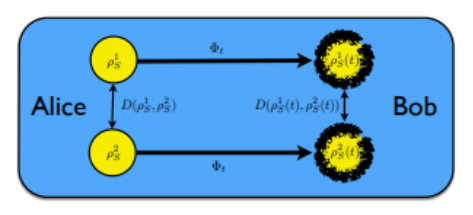
\includegraphics[width=0.7\linewidth]{pictures/state_alice_bob.png}
    \caption{Схема передачи состояния от Алисы к Бобу. Алиса готовит два различных состояния
    $\rho^{1}_{S}$ и $\rho^{2}_{S}$, которая передается по динамической карте с шумом
    $\Phi_{t}$, таким образом, сокращая доступную информацию Бобу. Потеря различимости количественно
    определяется расстоянием следа $D(\rho^{1}_{S}, \rho^{1}_{S})$.~\citep{breuer2016colloquium}}
    \label{fig:state_from_alice_to_bob}
\end{figure}
В тот момент, когда система просто теряет информацию, имеет случай марковского процесса, а когда
система получает информацию, имеет случай немарковского процесса.
Получение информации связано с откликом окружающей среды на воздействие открытой квантовой системы,
что свидетельствует о наличии памяти у окружающей среды.

Примеры немарковких процессов присутствуют так же и в оптических процесах.
Частный пример тому связан с квантовым броуновским движением в оптическом резонаторе, который связан
с тепловым резервуаром.
В этом эксперименте установка имеет лазерный луч разделенный на сигнальный и на генераторный.
Генераторный луч попадает на микромеханический резонатор, который влияет на его биение.
Это биение влияет на фазу сигнального луча, который затем попадает на два фотодиода, которые регистрируют
изменение фазы~\citep{nonmark2017dynamics}.
Биение микрорезонатора сопровождается остаточными осциляциями, которые могут служить «памятью» процесса.
Этот пример приведен на рисунке~\ref{fig:nonmark_brown}.
\begin{figure}[h!]
    \centering
    \captionsetup{justification=centering}
    \begin{minipage}[h]{0.4\linewidth}
        \center{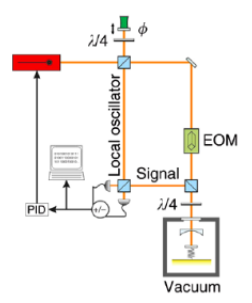
\includegraphics[width=1\linewidth]{pictures/nonmark_a.png} \\ а)}
    \end{minipage}
    \begin{minipage}[h]{0.5\linewidth}
        \center{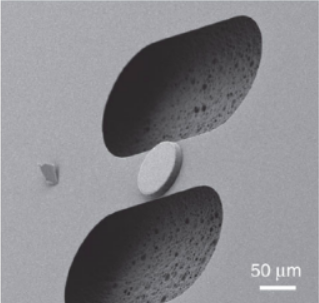
\includegraphics[width=1\linewidth]{pictures/nonmark_b.png} \\ б)}
    \end{minipage}
    \caption{a) Экспериментальная установка, состоящая из разделенного на сигнальный и генераторный
    лазерного излучения. Сигнальный луч получает фазу из-за движения механического резонатора.
    б) Сканирующая электронная микроскопия изображения тестируемого устройства~\citep{nonmark2017dynamics}}
    \label{fig:nonmark_brown}
\end{figure}

Результаты эксперимента показывают неомическую спектральную плотность и проявляют немарковский процесс~\citep{nonmark2017dynamics}.

%%%%%%%%%%%%%%%%%%%%%%%%%%%%%%%%%%%%%%%%%%%%%%%%%%%%%%%%%%%%%%%%%%%%%%%%%%%%%%%%%%%%%%%%%%%%%%%%%%%%
%%%%%%%%%%%%%%%%%%%%%%%%%%%%%%%%%%%%%%%%%%%%%%%%%%%%%%%%%%%%%%%%%%%%%%%%%%%%%%%%%%%%%%%%%%%%%%%%%%%%
\section{Принятие решения в квантовом формализме}

В процессе принятия решения на человека может воздействовать окружающая обстановка(внешние возбудители).
Окружающая обстановка влияет на человека через органы чувств: зрение, слух, обаняние, физические воздействия.
Органы чувств передают информацию об окружающей обстановке в головной мозг, где в дальнейшем
информация обрабатывается и сохраняется.
Эта информация в дальнейшем может участвовать в процессе мышления и иметь случайный характер, благодаря
чему принятие определенного решения может оказаться непредсказуемым.
Такое непредсказуемое решение ранее было рассмотрено в дилемме заключенного с наблюдаемым эффектом дизъюнкции.
В физике эффект дизъюнкции присутствует в явлениях интерференции.
В том и в другом случае наблюдается общий вклад каких-либо вариантов событий.
Таким образом можно рассматривать когнитивный парадокс в дилемме заключенного как являение интерференции в физике.
Подобно этому можно привести сравнение человека как квантовой системы (атома), а окружающего его
возбудителя как резервуар (гармонические осцилляторы), согласно теории открытых квантовых систем.
При этом энергия спонтанного излучения атома, поглощенная резервуаром, превращается в осцилляции
резервуара, которые могут иметь поведение как марковского так и немарковского процесса.
Мода спонтанного излучения атома в резервуаре описывается гамильтонианом:
\begin{equation}
    H_{a} = \hbar \omega a^{\dagger} a
\end{equation}
где $a, a^{\dagger}$ - операторы рождения уничтожения моды, $\hbar$ - постоянная Планка, $\omega$ -
частота моды излучения.
Поглощения резервуаром обусловлены связью квантовой системы и резервуара, поэтому если энергия от
квантовой системы передается резервуару, то через некоторое время оно за счет связи может вернуться.
Такой же эффект можно наблюдать в классической физике, когда слабая связь между двумя классическими
осцилляторами позволяет усиливать частоту одного осциллятора за счет другого.
Марковский процесс проявляется в случае потери связи квантовой системы с резервуаром, тоесть атом
не получает энергию обратно от резервуара.
Немарковский процесс проявляется в случае влияния резервуара на квантовую систему через связь, тоесть
атом получает энергию обратно от резервуара.
Осцилляторы совершают упругие колебания и таким образом их можно представить как элементы некоторой
кристаллической решетки~\citep{barnett2002methods}.
Эти упругие колебания можно проквантовать также как электромагнитные колебания в диэлектрике, которые
описываются статистикой Бозе-Эйнштейна и называются фононами.
Гамильтониан для фононов имеет вид:
\begin{equation}
    H_{b} = \sum_{j} \hbar \omega_{j} b_{j}^{\dagger} b_{j}
\end{equation}
где $b, b^{\dagger}$ - операторы рождения уничтожения фононов(колебаний резервуара), $\hbar$ - постоянная
Планка, $\omega_{j}$ - частоты фононов резервуара.
В случае если частоты фононов резервуара расположены очень плотно друг другу, то сумму можно заменить
на знак интеграла.
Если твердое тело (диэлектрик) находится в тепловом равновесии, то его распределение атомов по энергиям
описывается уравнением Больцмана.
В таком случае множество осцилляторов описываются оператором плотности в момент времени $t = 0$:
\begin{equation}
    \rho_{b} (0) = \prod_{j=1}^{N} \rho_{j} (0)
\end{equation}
где $N$ - число атомов в резервуаре, $\rho_{j} (0) = (1-exp(-\lambda_{j})) exp(-\lambda b_{j}^{\dagger} b_{j})$,
$\lambda_{j} = \frac{\hbar \omega_{j}}{kT}$.
Таким образом гармонические осцилляторы, которые находятся в тепловом равновесии с резервуаром
температурой $T$, аналогичны поведению фононам~\citep{barnett2002methods}.
Общий гамильтониан квантовой системы и системы осцилляторов записывается в следующем виде:
\begin{equation}
    H_{0} = \hbar \omega a^{\dagger} a + \sum_{j} \hbar \omega_{j} b_{j}^{\dagger} b_{j}
\end{equation}
Этот гамильтониан описывает~навзаимодействующие, несвязанные системы резервуара и атома.
Для учета~связи~необходимо внести гамильтониан взаимодействия подсистем.
Для ионных кристаллов такое взаимодействие обусловлено передачей электромагнитного поля.
Гамильтониан взаимодействия, который сохраняет полную энергию системы, описывается следующим образом:
\begin{equation}
    H_{1} = \sum_{j} \hbar (k_{j} a^{\dagger} b_{j} + k_{j}^{*} a b_{j}^{\dagger})
\end{equation}
где $k_{j}$ - коэффициенты связи.
Обычно коэффициенты связи считаются малыми по сравнению с частотой моды излучния и упругих колебаний
резервуара, поскольку зависят от характера взаимодействия систем~\citep{barnett2002methods}.
Введенные параметры очень сильно влияют на связь между осцилляторами резервуара и атома, если частота
упругих колебаний резрвуара приблизительно равна частоте моды излучения.
Гамильтониан взаимодействия не содержит члены вида: $k_{j} a^{\dagger} b_{j}^{\dagger}, k_{j}^{*} a b_{j}$,
поскольку их вклад во взаимодействие равен нулю.
В итоге имеем полный гамильтониан, который описывает взаимодействие моды излучения и осцилляторами(фононами):
\begin{multline}
    H = H_{0} + H_{1} = \hbar \omega a^{\dagger} a + \sum_{j} \hbar \omega_{j} b_{j}^{\dagger} b_{j} +
    \sum_{j} \hbar (k_{j} a^{\dagger} b_{j} + k_{j}^{*} a b_{j}^{\dagger})
\end{multline}

%%%%%%%%%%%%%%%%%%%%%%%%%%%%%%%%%%%%%%%%%%%%%%%%%%%%%%%%%%%%%%%%%%%%%%%%%%%%%%%%%%%%%%%%%%%%%%%%%%%%
%%%%%%%%%%%%%%%%%%%%%%%%%%%%%%%%%%%%%%%%%%%%%%%%%%%%%%%%%%%%%%%%%%%%%%%%%%%%%%%%%%%%%%%%%%%%%%%%%%%%
%\section{Дилемма заключенного в квантовом формализме}

Для дилеммы заключенного каждая квантовая модель рассматривается в гильбертовом пространстве, которое
может быть бесконечномерным.
Для системы из двух игроков достаточно конечного пространства.
Определение размерности зависит от количества исходов игры и для этого необходимо определить какие
есть варианты развития событий.
В задаче дилеммы заключенного участвуют двое игроков $G_{1}$ и $G_{2}$ , у каждого из которых есть по два возможных
варианта выбора это сдать и не сдавать, обозначим как вектора в гильбертовом пространстве
$\vert 0 \rangle$ и $\vert 1 \rangle$, соответственно.
Тогда, функцию состояния каждого игрока можно описать с помощью следующей формулы:
\begin{equation}
    \vert \psi \rangle_{j} = \sum_{j=0,1} a_{j} \vert j \rangle
\end{equation}
где $a_{j}$ - коэффициент проекции вектора $\vert j \rangle$.

Такую~функцию~можно~представить~с~помощью двумерного гильбертова пространства $\mathbb{C}^{2}$.
Квадрат модуля коэффициента $\vert a_{j} \vert^{2}$ имеет смысл как вероятность выбора одного из
векторов $\vert 0 \rangle$ или $\vert 1 \rangle$.
В таком пространстве базисы векторов двух игроков могут быть повернуты на угол друг относительно друга,
а значит в таком случае при выборе одинакового значения двух игроков, направление вектора состояния
будет различаться из-за различного ментального восприятия мира.
При использовании данной формулы можно определить вариант выбора одного игрока, однако на основе
выбора первого невозможно определить выбор другого, иначе говоря их решение не влияет на результат
другого, что в данной дилемме не всегда так, поскольку при повторении игры прошлый опыт влияет на
обоих игроков одновременно.
Поэтому необходимо определить другую функцию состояния, которая впоследствии позволит правильно
определить размерность гильбертова пространства.
Поскольку выбор двух игроков должен влиять друг на друга, то получается они имеют общую функцию
состояния, имеющая следующий вид:
\begin{equation}
    \vert \Psi \rangle_{j} = \sum_{k,l=0,1}^{1} a_{k,l} \vert kl \rangle
\end{equation}
из этой формулы так же видно, что у игроков имеется общее ментальное состояние, что как раз более
правдоподобно в реальном мире.
По аналогии из формулы выше для двумерного гильбертова пространства, $a_{k,l}$ – коэффициент
проекции вектора $\vert kl \rangle$, где $\vert kl \rangle$ – вектор выбора двух игроков
(всего их четыре $\vert kl \rangle$ $\vert kl \rangle$ $\vert kl \rangle$ $\vert kl \rangle$),
а квадрат коэффициента проекции $\vert a_{j} \vert^{2}$ имеет смысл как вероятность выбора исхода игры.
